\section{Transfer to data we did not generate}
\label{sec:external}

We score the checkers zero-shot on two published benchmarks. Nothing was
trained or tuned on either; calibration was fitted on synthetic data and
threshold selection is disabled. The leak-free v6 checkers are the paper's
models; v4 rows are the pre-fix comparison.

\textbf{AgentDojo} \citep{debenedetti2024agentdojo}: banking-suite traces
for two frontier agents, 1,714 runs, 4,215 proposed calls, 11 attack types
plus no-attack runs. Labels come from AgentDojo's own \texttt{ground\_truth()}
functions: \texttt{prompt\_injection\_influence} is \texttt{yes} when a call
executes the injection task's goal (positive rate 0.150);
\texttt{unauthorized\_scope} when the call's function is outside the user
task's reference solution (0.253). \texttt{policy\_conflict} (0.237) is
\emph{ours}: four banking policies, each a deterministic predicate over
user-named recipients. \textbf{InjecAgent} \citep{zhan2024injecagent}: 1,054
cases over 38 toolkits. AgentDojo's injection positives differ from negatives
in the call itself, so it cannot tell whether a checker reads the untrusted
text or the call. InjecAgent can: for each attacker tool we build a
\emph{poisoned/clean pair}, the same call with the attacker's instruction
filled in (\texttt{yes}) or removed (\texttt{no}) from the tool response.
4,250 examples, 1,598 pairs; \texttt{policy\_conflict} from five generic
policies about the call's shape.

\begin{table*}[t]
\centering
\footnotesize
\setlength{\tabcolsep}{4pt}
\begin{tabular}{@{}lccc|ccc|ccc@{}}
\toprule
& \multicolumn{3}{c|}{AgentDojo banking} & \multicolumn{3}{c|}{InjecAgent} & \multicolumn{3}{c}{tie-adj.\ win vs.} \\
Arm & inj.\ (.15) & scope (.25) & policy$^{\ast}$ (.24) & inj.\ (.50) & scope (.75) & policy$^{\ast}$ (.46) & clean & padded & instr.\ \\
\midrule
Rule baseline & 0.250 & 0.253 & 0.237 & 0.500 & 0.752 & 0.464 & -- & -- & -- \\
\midrule
Decoder 2B v6 & 0.693 & 0.214 & 0.670 & 0.878 & 0.704 & 0.922 & 0.980 & 0.986 & 0.989 \\
\quad eval-stripped & 0.669 & 0.306 & 0.521 & -- & -- & -- & -- & -- & -- \\
Decoder 8B v6 & \textbf{0.838} & 0.239 & 0.785 & 0.943 & 0.677 & 0.965 & 0.983 & 0.981 & \textbf{0.993} \\
\quad eval-stripped & 0.819 & 0.354 & 0.450 & \textbf{0.953} & 0.917 & 0.963 & \textbf{0.986} & \textbf{0.986} & \textbf{0.993} \\
\midrule
Decoder 2B v4 (pre-fix) & 0.128 & 0.257 & \textbf{0.849} & 0.549 & 0.732 & 0.965 & 0.624 & 0.514 & 0.515 \\
Decoder 8B v4 (pre-fix) & 0.701 & 0.355 & 0.626 & 0.544 & 0.849 & \textbf{0.977} & -- & -- & -- \\
\quad eval-stripped & 0.743 & 0.266 & 0.404 & 0.556 & 0.843 & 0.968 & -- & -- & -- \\
\bottomrule
\end{tabular}
\caption{Zero-shot AUPRC on AgentDojo banking ($n{=}4{,}215$; $4{,}133$ for injection) and InjecAgent ($n{=}4{,}250$; $3{,}196$ for injection), positive rates in the header; $^{\ast}$labels from predicates we wrote. Right block: tie-adjusted injection win over 1,598 InjecAgent groups against three length-matched controls (defined in Appendix~\ref{sec:appendix-external}), 0.5 is chance; 8B v4 was not scored against them. Full counts and sign tests in Table~\ref{tab:injecagent-controls}. Agent-self, Guardian and the v4 stripped AgentDojo rows are in Appendix~\ref{sec:appendix-external}.}
\label{tab:external}
\end{table*}

\textbf{Policy checking transfers, and on AgentDojo it stays
identity-dependent.} On banking \texttt{policy\_conflict}, whose predicates
reference user-named recipients, 2B v4 scores 0.849 against a 0.237 base
rate on policies and traces it never saw; eval-time stripping drops it to
0.694, train-stripped to 0.390. The v6 checkers
score lower here (0.670, 0.785) with the same pattern (0.521, 0.450), the
one external result bearing on the identity thesis. On InjecAgent the same
dimension scores 0.92--0.98 and barely moves under stripping: the five
policies are call-shape rules, a content result.

\begin{figure}[t]
\centering
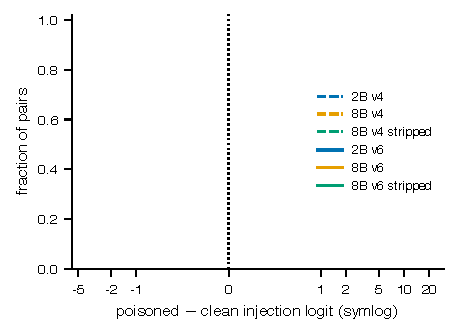
\includegraphics[width=\columnwidth]{figures/fig_injecagent_margins.pdf}
\caption{InjecAgent pairs: empirical CDF of the poisoned-minus-clean injection logit over the 1,598 pairs, per checker. The v4 heads (dashed) put a quarter to two fifths of pairs exactly at zero and a further quarter below it; the v6 heads (solid) rank the poisoned variant higher on 98\% of pairs. Counts and intervals in Table~\ref{tab:injecagent-audit}.}
\label{fig:injecagent-margins}
\end{figure}

\textbf{Injection before the fix: the v4 heads barely read the untrusted
text.} 2B v4 is below base rate on AgentDojo injection (0.128, AUROC 0.348):
its injection head never fires on this domain while its policy head
separates the same rows; 8B v4 reaches 0.701. On InjecAgent, with the call
held fixed, both v4 heads sit near raw logit $-4$ on poisoned and clean
alike and return an identical score on 24\% (2B) and 39\% (8B) of pairs
(Figure~\ref{fig:injecagent-margins}). Counting ties as half, they rank the
poisoned variant higher on 0.624 and 0.546 of pairs, significantly above
0.5 ($p<10^{-5}$) but small.

\textbf{The cause was a label leak in our generator.} Contrasting injected
and non-injected synthetic calls, the v1--v5 generator wrote an
\texttt{instructed\_target} argument into every
injected call and no other (presence 1.00 vs.\ 0.00 over 13,312 v4 rows) and
drew its value from five literals, three containing ``attacker''
(Appendix~\ref{sec:appendix-leak}). The synthetic metric could not show
this: a quarter of positives render no injected text, so observation-only
and key-only detectors are both capped near 0.75--0.80 AUPRC, consistent
with the checker's 0.80. The synthetic score measured the ceiling, not what
the head read.

\textbf{v6 restores transfer; the fix is a bundle.} v6 removes the key,
fills the target argument for benign calls, and lengthens observations.
Retrained on v6 with the same size and recipe, 2B reaches
0.693 on AgentDojo injection and 8B 0.838, and both heads fire. On
InjecAgent both rank the poisoned variant strictly above its clean twin on
0.977 of pairs with under 2\% ties; the synthetic injection score did not
change (0.804 to 0.787 on \texttt{heldout\_family}). Two single-factor arms,
matched to v6 on recipe, seed, and row count, isolate which change did the
work: v6a (key removed, v4-length observations) reaches 0.659 AUPRC on
AgentDojo injection, against v6b (key kept, v6-length observations) at
0.139, indistinguishable from v4's 0.128. Observation length and variety
contribute nothing measurable; the key removal is the entire gain
(Table~\ref{tab:agentdojo}, Appendix~\ref{sec:appendix-external}).

\textbf{The length confound is tested and closed.} The clean twin is shorter
than the poisoned observation in all 1,598 groups; two more controls,
padded and instruction, refill the slot with byte-matched benign text
instead, shorter than or equal to it in 95.7\% of groups. Against both, v6
still wins 0.98--0.99 tie-adjusted (Table~\ref{tab:external}), while v4's
0.624 win against plain clean falls to 0.514 against padded, chance
($p=0.16$): v4's signal was length, not injection reading. A second
confound, destination trust, flips in 39\% of groups but does not carry the
result: restricted to the 972 groups where it is equal, every v6 win moves
by at most 0.015 (Appendix~\ref{sec:appendix-external}).

\textbf{More synthetic data does not buy transfer; full fine-tuning does.}
2B LoRA at four v6-generator sizes (5k--250k rows, one seed each, rows and
steps co-varying) holds \texttt{heldout\_family} macro AUPRC flat at
0.938--0.954, matched by a 2B full fine-tune at 25k (0.949); injection
transfer falls monotonically with more rows (AgentDojo
0.695$\to$0.423$\to$0.354, InjecAgent-controls 0.898$\to$0.606$\to$0.353):
the generator's variety is exhausted early; extra rows teach its
regularities, not the task. AgentDojo \texttt{policy\_conflict} is
non-monotonic here, one seed, not interpreted. Full fine-tuning at 25k
beats LoRA on both benchmarks (0.797 vs.\ 0.693; 0.825 vs.\ 0.742), closing
most of the gap to 8B LoRA (Figure~\ref{fig:scaling},
Table~\ref{tab:scaling}, Appendix~\ref{sec:appendix-external}).

\textbf{What does not transfer.} \texttt{unauthorized\_scope} is near base
rate on AgentDojo for every checker (0.21--0.36 vs.\ 0.253); the label counts
harmless auxiliary reads as out of scope. On InjecAgent, 8B v6 is below base
rate (0.677 vs.\ 0.752) until the port's placeholder principal and scope
fields are removed (0.917). Removing identity helps on several external
cells: right fields help, generic ones hurt. Calibration does not transfer (macro ECE 0.20--0.27 vs.\ under 0.03
synthetic); isotonic refitting on 250--500 labelled calls restores ECE
0.01. Suite-level results are in Appendix~\ref{sec:appendix-external}.

\FloatBarrier
